\begin{englishtitle} % Настраивает LaTeX на использование английского языка
% Этот титульный лист верстается аналогично.
\title{One problem of achieving an incompletely known target set}
% First author
\author{Alexandr Barinov} 

\institute{Chelyabinsk State University, Chelyabinsk,Russia\\
  \email{barinovalexmih@mail.ru}}
 % \and
%Affiliation, City, Country\\
%\email{email@example.com}}
% etc

\maketitle

\begin{abstract}
We consider the problem of passing a maze with exits unknown in advance, namely, in the maze there are $2$ exits, one of which is real and the other false. Which of the outputs is real at the initial moment of time is unknown. Subsequently, at each step, with probability $p$, the position of the real exit is revealed, so the goal of the decision maker is to move along a trajectory from which he can get to any exit as long as possible.

\keywords{optimal control, finding a path in a maze, Lee algorithm} % в конце списка точка не ставится
\end{abstract}
\end{englishtitle}

\iffalse
%%%%%%%%%%%%%%%%%%%%%%%%%%%%%%%%%%%%%%%%%%%%%%%%%%%%%%%%%%%%%%%%%%%%%%%%
%
%  This is the template file for the 6th International conference
%  NONLINEAR ANALYSIS AND EXTREMAL PROBLEMS
%  June 25-30, 2018
%  Irkutsk, Russia
%
%%%%%%%%%%%%%%%%%%%%%%%%%%%%%%%%%%%%%%%%%%%%%%%%%%%%%%%%%%%%%%%%%%%%%%%%


\documentclass[12pt]{llncs}  

% При использовании pdfLaTeX добавляется стандартный набор русификации babel.

\usepackage{iftex}

\ifPDFTeX
\usepackage[T2A]{fontenc}
\usepackage[utf8]{inputenc} % Кодировка utf-8, cp1251 и т.д.
\usepackage[english,russian]{babel}
\fi

\usepackage{todonotes} 

\usepackage[russian]{nla}

\begin{document}
\fi

\title{Одна задача достижения не полностью известного целевого множества}%\thanks{Работа выполнена при поддержке РФФИ (РНФ, другие фонды), проект \textnumero~00-00-00000.}}
% Первый автор
\author{А.~М.~Баринов
}

% Аффилиации пишутся в следующей форме, соединяя каждый институт при помощи \and.
\institute{Челябинский государственный университет (ФГБОУ ВО <<ЧелГУ>>), Челябинск, Россия \\
  \email{barinovalexmih@mail.ru}
 % \and   % Разделяет институты и присваивает им номера по порядку.
%Институт (название в краткой форме), Город, Страна\\
  %\email{email@example.com}
% \and Другие авторы...
}

\maketitle

\begin{abstract}
Рассматривается задача о прохождении лабиринта с неизвестными заранее выходами, а именно в лабиринте имеется $2$ выхода, один из которых настоящий, а другой ложный. Какой из выходов настоящий в начальный момент времени неизвестно. В дальнейшем, на каждом шагу с вероятностью $p$ открывается положение настоящего выхода, поэтому цель ЛПР ---  движение по траектории, из которой он как можно дольше может попасть в любой выход.

\keywords{оптимальное управление, поиск пути в лабиринте, алгоритм Ли } % в конце списка точка не ставится
\end{abstract}

%\section{Основные результаты} % не обязательное поле

Задачи нахождения алгоритмов выбора пути в условиях неопределенности исследовались во многих рабодах, например\cite{bar1,bar2}. В докладе рассматривается следующая задача.\\

Пусть позиция $x$ задается вектор-столбцом $x=(x_1,x_2)'$ где $x_1\in \{1,2,\ldots,n\},$ $x_2\in \{1,2,\ldots,m\}$, штрих означает операцию  транспонирования.

Множество всех позиций задачи обозначим
\begin{center}
 $X=\{x=(x_1,x_2)' || x_1, x_2\in \mathbb{N}, x_1\leq n, x_2\leq m\}$,
\end{center}
а множество допустимых позиций $P \subseteq X$.

Рассматривается задача с дискретным временем $t$, где $t\in\{0,1,2,\ldots,T\}$.
Положение системы в момент времени $t+1$  $(t \in 0, \ldots,T-1)$ задается системой разностных уравнений
\begin{equation} \label{eq1}
		\begin{cases}% создание окружения для систем уравнений
			x_1(t+1)=x_1(t)+u_1(t),\\
			x_2(t+1)=x_2(t)+u_2(t),\\
		\end{cases}
\end{equation}
где управление $u(t)$ в момент времени $t$ имеет вид
\begin{equation} \label{eq2}
u(t)= (u_1(t),u_2(t))', \;\;\;\; u_i(t) \in \{-1,0, 1\} \;\; (i=1,2).
\end{equation}

Система (1), (2) описывает перемещение точки, расположенной в клетке прямоугольной сетки в одну из восьми соседних клеток, либо отсутствие перемещения (см. рис.\ref{fig1}).
\begin{figure}[h]
\centering
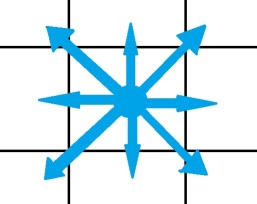
\includegraphics[width=0.4\linewidth]{ris.jpg}
\caption{Направления перемещения}
\label{fig1}
\end{figure}
Такая система, с учетом множества допустимых позиций, может трактоваться как движение точки по лабиринту.

Задано начальное положение системы
\begin{equation} \label{eq3}
 x(0)=(x_1(0),x_2(0))'=x^0=(x_1^0,x_2^0)'.
\end{equation}

Предполагается, что cистема в момент времени $T$ должна попасть в целевую позицию (выход из лабиринта), о которой известно, что это либо $x^*$, либо $x^{**}$ (то есть должно быть выполнено одно из условий $x(T)=x^*$, или $x(T)=x^{**}$, но какое -- заранее неизвестно.

На каждом шаге с вероятностью $p$ становится известно настоящее положение выхода.

Пусть момент времени $T_1<T$ --- это последний момент времени, в который ЛПР, двигаясь по некоторой траектории, может привести систему как в положение $x(T)=x^*$, так и в $x(T)=x^{**}$.

Вероятность того, что ЛПР откроется положение настоящего выхода к моменту времени $T_1$ будет 
\begin{center}
$P_{T_1}=p+(1-p)p+{(1-p)^2}p+\ldots+{(1-p)^{{T_1}-1}p}$.
\end{center}
Перед ЛПР стоит следующая задача
\begin{center}
$P=P_{T_1}+\frac{1-P_{T_1}}{2}\rightarrow max$,
\end{center}
что равносильно 
\begin{equation} \label{eq4}
T_1 \rightarrow max .
\end{equation}


Решением задачи оптимального управления (1)--(4) будем называть пару $(\hat{u}, \hat{x}(\cdot))$, где
оптимальное управление
$$
\hat{u}=(\hat{u}(0),\ldots ,\hat{u}({{T}_{1}}-1),({{{\hat{u}}}^{*}}({{T}_{1}}),{{{\hat{u}}}^{*}}({{T}_{1}})),\ldots ,({{{\hat{u}}}^{*}}(T-1),{{{\hat{u}}}^{**}}(T-1))),
$$
а, определяемая этим управлением, оптимальная траектория
$$
\hat{x}(\cdot)=(\hat{x}(0),\ldots ,\hat{x}({{T}_{1}}),({{{\hat{x}}}^{*}}({{T}_{1}}+1),{{{\hat{x}}}^{**}}({{T}_{1}}+1)),\ldots ,({{{\hat{x}}}^{*}}(T),{{{\hat{x}}}^{*}}(T))).
$$

В докладе предлагается алгоритм решения задачи (1)--(4) и приводятся результаты численного моделирования.


\setcounter{equation}{0}
\setcounter{figure}{0}

\small


\begin{thebibliography}{9} % или {99}, если ссылок больше десяти.
\bibitem{bar1} Кирильченко А.А. Обоснование алгоритмов выбора пути в условиях неопределенности  // Препринт Ин-та прикл. матем. им. М.В. Келдыша АН СССР, 1991, \textnumero~108, 25~с.

\bibitem{bar2} Бакиров А. К., Кирильченко А. А. Исследование особых ситуаций для задачи выбора пути в условиях неопределенности // Препринты ИПМ им. МВ Келдыша.  2001.   \textnumero~31.

\end{thebibliography}

% После библиографического списка в русскоязычных статьях необходимо оформить
% англоязычный заголовок.




%\end{document}

